Due to the reasons discussed in section \ref{sec:StateOfTheArt}, the TRITIUM detector developed used to measure the tritium levels of water samples is a scintillator detector. It consists in a chain of three main elements:

\begin{itemize}

\item{} The scintillator, that is the material in charge of detecting the tritium event. A general particle (tritium in our case), ionizing radiation, hit this material and deposits part of their kinetic energy (or all, as in our case) in it through ionization and excitation processes. Part of this energy deposited is converted in photons, generally in the visible range\footnote{The visible range is made up by photons with a wavelength between $380~\nm$ and $750~\nm$}.

The produced photons produced carry information about the particle detected, like its energy, type, etc.

\item{} The photosensor, which is the part of the detector in charge of detecting the photons produced by the scintillator that reach it (the more scintillated photons arrive to your photosensor, the better signal you have in your detector). 

The most used photosensor in nuclear physics are PMTs and SiPMs which detects the photons produced in the scintillator (with an efficiency) and transforms it in electrons which are multiplied with a factor of around $10^6$. This millions of electrons form a electronic pulse the properties of which has information of the photons that has been detected.

\item{} The electronic system, which is the part of the scintillator detector in charge of processesing and analyzing (first analogically and then digitally) this electrical pulse of the photosensor. The output of the electronic system is useful information about the event detected such as a number, for instance the activity, or some kind of spectrum like energy spectrum.

\end{itemize}

In Figure \ref{fig:ScintillatorDetector} a scheme of a scintillation detector is shown. There, the scintillator material detects ionizing radiation and produces photons that will be guided by the reflector and the light guide to the photosensor. There, some of the photons that reach the sensible part of the photosensors will be converted and multiplied into millions of electrons that will form a electronic pulse. The output signal of the photosensor (electronic pulse) will be processed and analyzed by the corresponding electronics:

\begin{figure}[hbtp]
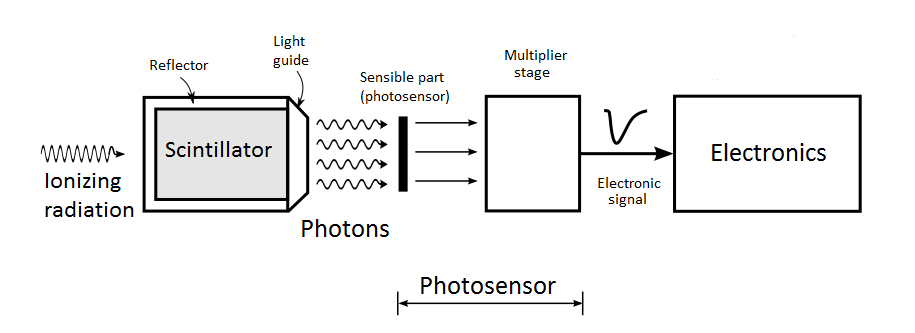
\includegraphics[scale=0.6]{3DesignPrinciples/32Tritium_detector/ScintillatorDetector.png}
\centering
\caption{Scheme of the scintillator detector\label{fig:ScintillatorDetector}}
\end{figure}
